%%!TEX root = document.tex

The project's source code, benchmark scripts, analysis code and plots are provided in an open source  \href{https://bitbucket.org/bcardoen/csrm}{repository}. Additional results, left out here due to space constraints are covered in \href{https://bitbucket.org/bcardoen/csrm/src/9de4b990ce27bbaeb885203f82a76635d8d92473/thesis/thesis/MsCThesisBenCardoen.pdf?at=master&fileviewer=file-view-default}{work}.
The experiments were performed on an Intel Xeon E5 2697 processor with 64GB RAM, with Ubuntu 16.04 LTS.  The experiments use a fixed seed in order to guarantee reproducibility. For the parallel experiments we use 25 processes.
%Where relevant we specify the parameter configuration.
 
\paragraph{Benchmark problems}
Recent work on the convergence of GP-based SR \cite{SRAccur, SRBaseline} featured a set of benchmarks that pose convergence problems for SR implementations. 
These 15 benchmarks use at most five features and are non-linear arithmetic expressions using standard base functions : (sin, cos, tan(h), log,$a^x$, /, *, modulo, abs, min, max, +, -). CSRM does not know in advance which features are used. It only assumes that each problem is a function of maximum 5 features, testing the robustness of the algorithm.

\paragraph{Experiment setup}
Each process has a population of 20 expression trees with an initial depth of 4, max depth of 8, executes 20 phases of 20 runs or generations with an archive size of 20 expressions. Per phase, the 4 best expressions are archived. The benchmark functions have at most 5 features with 20 sample points in the range [1,5]. The Grid and Tree topology share their best expression per link, the Random topology shares 2 expressions per link. We used 25 processes, resulting in respectively 400, 15, 50 expressions being sent per phase. The random topology in this case contains is a disconnected set of 2 cycles.

At the end of an experiment, the best 20 expressions from all processes are collected and scored. We measure the fitness on the training data, and the fitness on the validation data. 
Finally, we record the mean fitness values of the best 5 expressions, both on the training and validation data, as convergence rate.
The mean is restricted to the upper quarter of the population specifically to measure how the best expressions are distributed. %LW: dit begrijp ik net... 
% BC : De population mean is gevoelig aan outliers, e.g. 0.01, 0.02, 0.9,1,1,1 in edge cases (0.01 best, 1 worst), dus ik neem de mean van de best x om naar de 'effective subpopulation' te kijken.
This measure records the convergence more accurately as the fittest expressions drive the convergence rate, or put differently, it ignores the effect outliers would otherwise have on the mean. 
Fitness values fluctuate strongly across test problems and topologies. The results are presented in relative to the Tree topology to measure a relative gain or loss in orders of magnitude.
% on a negative logarithmic scale : $f_t = -\log_{10}(f)$ where f is the ratio of the best fitness values. 
%LW: the scale is not relevant is you present a ratio. It is used for both measures... // agreed


%\subsubsection{Results}
\paragraph{Convergence}


\begin{figure}
    \label{fig:ckfold}
	\begin{subfigure}{0.5\textwidth}\label{fig:csrmkfold}
    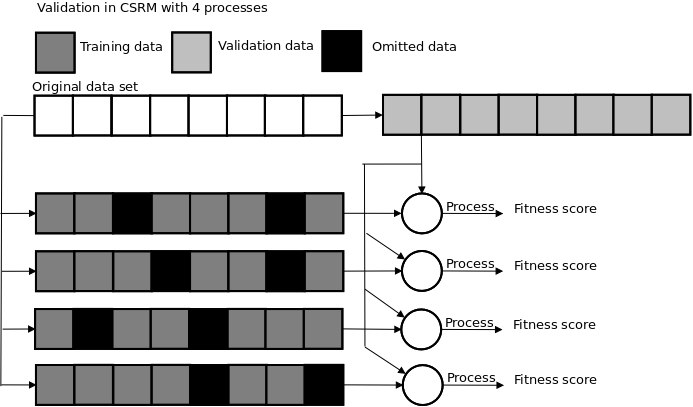
\includegraphics[width=\textwidth,height=\textheight,keepaspectratio]{figures/validationcsrm.png}
    \caption{Approximation of k fold cross validation \\with parallel processes, k = 4,  r = $\frac{3}{4}$.}
    \end{subfigure}
	\begin{subfigure}{0.5\textwidth}    \label{fig:kfold}

    \centering
    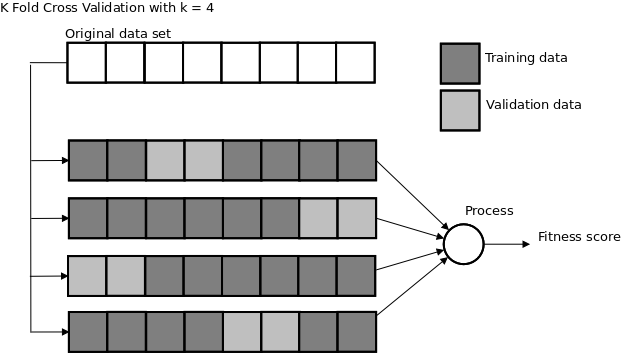
\includegraphics[width=\textwidth,height=\textheight,keepaspectratio]{figures/kfold.png}
    \caption{Visualization of k fold cross validation with k = 4.}
    \end{subfigure}%
    \caption{K fold cross validation approximation in CSRM.}
 \end{figure}
 
 \begin{figure*}
    \centering
    \begin{subfigure}{0.5\textwidth}
    \centering
        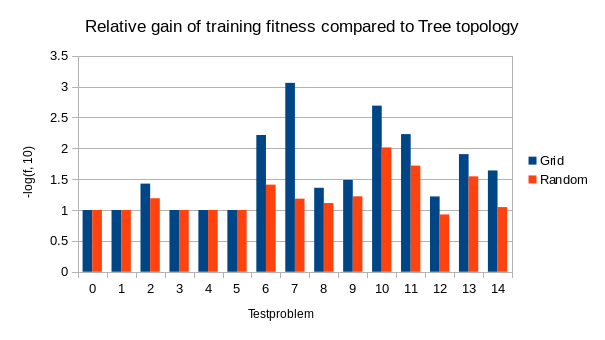
\includegraphics[width=0.6\linewidth]{figures/distributedbesttraining.png}
        \caption{Relative gain in best fitness of training data}
    \end{subfigure}%
    \begin{subfigure}{0.5\textwidth}
    \centering
        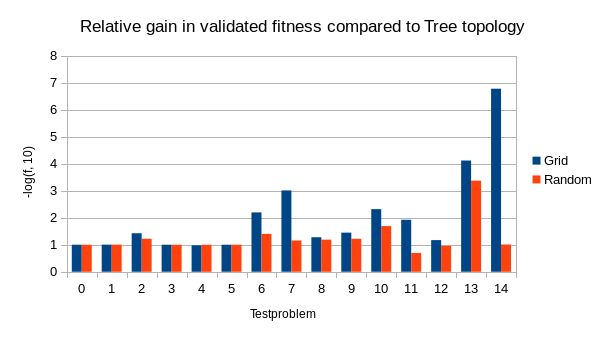
\includegraphics[width=0.6\linewidth]{figures/distributedbestvalidated.png}
        \caption{Relative gain in best fitness on full data.}
    \end{subfigure}
        \begin{subfigure}{0.5\textwidth}
    \centering
        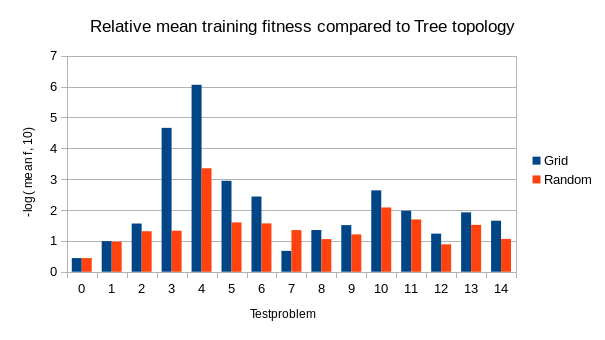
\includegraphics[width=0.6\linewidth]{figures/distributedmeantraining.png}
        \caption{Relative gain in mean fitness on training data.}
    \end{subfigure}%
    \begin{subfigure}{0.5\textwidth}
    \centering
        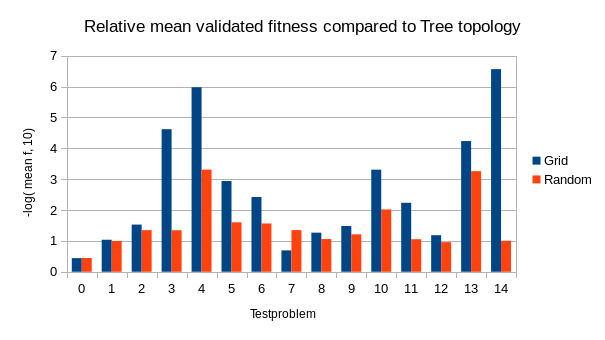
\includegraphics[width=0.6\linewidth]{figures/distributedmeanvalidated.png}
        \caption{Relative gain in mean fitness on full data.}
    \end{subfigure}
    \caption{Convergence differences between topologies.}
    \label{fig:distributedresults}
\end{figure*}

%Figure \ref{fig:distributedresults} shows large differences in the fitness based on the topology. 
For the best fitness, the first 5 benchmarks, with exception of the second, all have identical values on training and validation data. The processes converged to zero fitness values for these problems, hence the identical results. 
The fitness results on the training data, presented in Figure \ref{fig:distributedresults}a, indicate that the Grid and Random topology have superior convergence characteristics compared to the Tree topology, with Grid outperforming Random on more than half of the benchmarks. When we look at the fitness values on the validation data in Figure \ref{fig:distributedresults}b, we observe more nuanced results. Overall, the Grid topology is the best choice regarding best fitness values and the Random topology sometimes performs inferior compared to the Tree topology (e.g. benchmark 11 and 12). If we look at the mean fitness values on training and validation data, the Tree topology outperforms the Grid and Random topology on 2 benchmarks. However, the Grid topology performs still the best for most problems, with the exception of benchmark 7 where the Random topology dominates. The similarity between the results of the training and validation data, both for the best and mean fitness, indicates a good predictive capability since overfitting would result in a reverse patterns for the training and validation data. 

\paragraph{Measuring Overhead}
Cycles in the topology lead to excessive synchronization and serialization. We measure the mean execution time for benchmark 6, which leads to different convergence characteristics based on the topology, making this a good testcase. The processes will communicate 25 times. 
The runtime of one phase depends on the number of generations, population size and depth ranges of the expressions. 
Ideally, we would like for a user to choose these parameters based on the problem at hand and not be constrained by synchronization considerations. To compare the three topologies, we use the disconnected or 'none' topology as a reference point, as it has zero synchronization overhead and has an ideal speed-up of n, where n is the processcount. From the synchronization overhead we can then derive the speed-up each of the topologies is able to offer. In practice even the 'none' topology will have some synchronization overhead, as the root process has to collect all results.
Measuring communication overhead becomes hard if the runtime of a single phase is very long. If they are is too short, overhead dominates the entire runtime and it will unfairly penalize topologies with cycles forcing them to serialize. 

\begin{figure*}
    \centering
    \begin{subfigure}{0.5\textwidth}
    \centering
        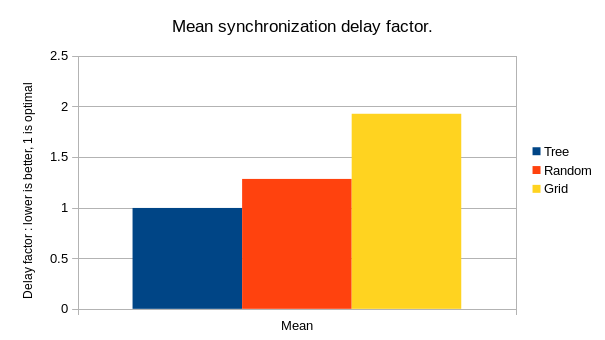
\includegraphics[width=0.7\linewidth]{figures/distributeddelaymean.png}
        \caption{Mean synchronization delay factor.}
    \end{subfigure}%
    \begin{subfigure}{0.5\textwidth}
    \centering
        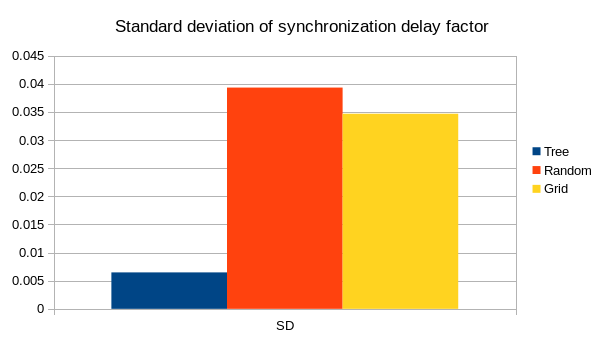
\includegraphics[width=0.7\linewidth]{figures/distributeddelaysd.png}
        \caption{Standard deviation of \\synchronization delay factor.}
    \end{subfigure}
    \caption{Synchronization overhead introduced by topologies.}
    \label{fig:distributeddelayresults}
    \end{figure*}
    
Figure \ref{fig:distributeddelayresults} shows that the Tree topology has almost no delay caused by synchronization. This is due to the delay tolerance we have built in in our implementation. The Random topology has an average delay factor of 1.3 and the Grid topology has an average delay factor of nearly 2. This is easily translated in terms of speed-up. As such, the Tree topology will have near linear speedup, a Grid topology roughly half of that and a Random topology will have an intermediate speed-up. The standard deviation on the speed-up for the Tree topology is significantly smaller indicating a predictable speed-up. 
It should be noted that selecting a different benchmark will lead to differing convergence characteristics, which in turn can mask synchronization effects. However, covering all benchmarks with all possible configurations is outside the computation scope of this work. 

%LW: do the performance results of the other benchmarks show the same message? If so, please mention this, and refer to the thesis. If not, please explain why...
%BC : You're right, but it's impossible to test all cases. So I have the implication (Topology -> Speedup) but this depends on the problem instance, which depends on the configuration. So all I can say is that our assumption is not disproved by this sample problem. E.g. more difficult or easier problems would actually mask or underline the synchronization effects.

